\documentclass[14pt,a4paper]{article}
\usepackage[14pt]{extsizes}
\usepackage[left=1.5cm, right=1.5cm, top=1.5cm, bottom=1.5cm]{geometry}
\usepackage[utf8]{inputenc}
\usepackage[T2A]{fontenc}
\usepackage[english, russian]{babel}
\usepackage{amsmath,amsfonts,amssymb,amsthm,mathtools} 
\usepackage{amsfonts}
\usepackage{amssymb}
\usepackage{titleps}
\usepackage{hyperref}
\usepackage{float}
\usepackage{graphicx}
\usepackage{multirow}
\usepackage{hhline}
\usepackage{wrapfig}
\usepackage{tikz}
\usepackage{pgfplots}
\usepackage{xcolor}
\usepackage{subfig}
\usepackage{upgreek}
\usepackage{bm}
\usepackage{longtable}


\newcommand{\w}[1]{\text{#1}}
\newcommand{\und}[1]{\underline{#1}}
\newcommand{\img}[3]{
	\begin{figure}[H]
	\begin{center}
	\includegraphics[scale=#2]{#1}
	\end{center}
	\begin{center}
 	\textit{#3}
	\end{center}
	\end{figure}
}
\newcommand{\aw}[1]{
	\begin{center}
	\textit{#1}
	\end{center}
	\n
}
\newcommand{\be}[1]{
	\begin{center}
	\boxed{#1}
	\end{center}
}
\newcommand{\beb}[1]{
	\begin{equation}
	\boxed{#1}
	\end{equation}
}
\newcommand{\eb}[1]{
	\begin{equation}
	#1
	\end{equation}
}
\newcommand{\n}{\hfill \break}
\newcommand{\x}{\cdot}

\begin{document}
\section*{Работа 4.7.3}	
\section*{Изучение поляризованного света}
\subsection*{Киркича Андрей, Б01-202, МФТИ}
\textbf{Цель работы: }
ознакомление с методами получения и анализа поляризованного света.
	\n\n
	\textbf{В работе используются: }
оптическая скамья с осветителем; зелёный светофильтр; два поляроида; чёрное зеркало; полированная эбонитовая пластинка; стопа стеклянных пластинок; слюдяные пластинки разной толщины; пластинки в 1/4 и 1/2 длины волны; пластинка в одну длину волны для зелёного света (пластинка чувствительного оттенка).

\section*{Теоретические сведения}
\subsection*{Типы поляризации}
%
%В зависимости от характера изменения ориентации пары векторов $\bm{E}$ и $\bm{H}$ в плоскости, перпендикулярной лучу $\bm{S}$, различают естественный и поляризованный свет. Если ориентация векторов $\bm{E}$ и $\bm{H}$ в волне хаотически изменяется во времени, так что в плоскости, перпендикулярной лучу S, все
%направления оказываются в среднем равноправными, свет называется \textit{естественным (неполяризованным)}. В \textit{линейно поляризованной} световой волне пара векторов $\bm{E}$ и
%$\bm{H}$ не изменяет с течением времени своей ориентации. В \textit{эллиптически поляризованной} световой волне конец вектора
%$\bm{E}$ (в данной точке пространства) описывает некоторый эллипс.
%
%\n\n
%Часто бывает удобно проектировать $\bm{E}$ в некоторой точке на два взаимно перпендикулярных направления. Если исходная волна была поляризованной, $E_x$
%и $E_y$ когерентны между собой и могут быть
%записаны в виде
%\[E_x = E_{x0} \cos (kz - \omega t)\]
%\[E_y = E_{y0} \cos (kz - \omega t - \varphi)\]
%
%Уравнения Максвелла можно разделить на две независимые системы:
%\begin{figure}[H]
%\centering
%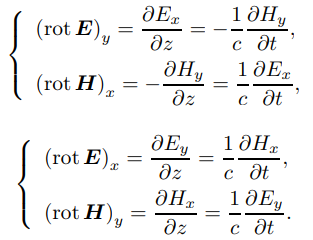
\includegraphics[width=6cm]{1.png}
%\end{figure}
%\n
%Частным случаем решения являются монохроматические волны:
%\[E_x = H_y = A_x \cos (\omega t - kz + \varphi_x),\]
%\[E_y = -H_x = A_y \cos (\omega t - kz + \varphi_y).\]
%\n
%В любой точке пространства концы векторов $\bm{E}$ и $\bm{H}$ в каждой из этих
%волн движутся по отрезкам прямых линий в плоскости ($E_x, E_y$), поэтому они называются \textit{линейно поляризованными}.
%\n\n
%Если обе описанные выше монохроматические волны распространяются одновременно, то концы векторов $\bm{E}$ и $\bm{H}$ движутся
%по эллипсам в плоскости ($E_x, E_y$) - \textit{эллиптическая поляризация}.
%\n\n
%Для квазихроматического света (может рассматриваться как последовательность независимых монохроматических цугов, между которыми происходит случайный сбой фазы) возможны три случая - поляризация наравне с монохроматическим (поляризация не меняется от цуга к цугу), неполяризованный свет (случайные и независимые изменения поляризации цугов) и частичная поляризация (есть преимущественное направление). Такая классификация справедлива и для немонохроматического света.
Пусть есть монохроматическая волна, вектор $\bm{E}$ колеблется по прямой линии в плоскости, перпендикулярной направлению распространения волны $\bm{k}$. Такую поляризацию называют \textit{линейной}.
\n\n
Если две монохроматические волны распространяются одновременно с некоторым сдвигом фаз, то конец суммарного вектора $\bm{E}$ будет двигаться по эллипсу (частные случаи - окружность, отрезок). Такая поляризация называется \textit{эллиптической}.
\subsection*{Получение поляризованного света}
Устройства, с помощью которых из естественного света получают
поляризованный, называются \textit{поляризаторами}. Есть несколько способов получить поляризованный свет:
\begin{itemize}
\item \textit{Дихроизм} -  способность вещества поглощать свет по-разному в зависимости от его поляризации. \textit{Поляроид} - прозрачная плёнка, в которую внедрено множество игольчатых кристаллов, причём они ориентированы преимущественно в одном направлении. Она сильно поглощает свет, плоскость поляризации которого перпендикулярна направлению выравнивания кристаллов, но слабо поглощает свет, плоскость поляризации которого параллельна направлению выравнивания.
\item \textit{Двойное лучепреломление} - результат зависимости коэффициента преломления (и угла преломления) от поляризации световой волны в анизотропных кристаллах.
\item \textit{Поляризация света при отражении и преломлении} - происходит на границе изотропного диэлектрика. Энергетический коэффициент отражения плоской волны с направлением, параллельным плоскости падения, может занулиться, когда угол между направлениями распространения отражённой и преломлённой волн прямой. В этом случае свет поляризуется.
\item \textit{Рассеяние света} - происходит на частицах пыли, молекулах газа или на атомах в кристаллах. При этом рассеянная волна оказывается поляризованной.
\end{itemize}

\subsection*{Наблюдение и анализ поляризованного света}
Используется поляризатор, который принято называть \textit{анализатором}.
\n\n
%При прохождении через анализатор линейно поляризованного света выполняется \textit{закон Малюса}, выражающий интенсивность прошедшей волны:
%\[I = I_0 \cos ^2 \varphi,\]
%\n
%где $\varphi$ - угол между направлением электрических колебаний анализируемой волны и разрешённым направлением поляризатора.
%\n\n
С помощью одного анализатора невозможно отличить неполяризованный свет от поляризованного по кругу. Можно использовать набор пластинок, вырезанных параллельно главной оптической оси кристалла, которые помещают перед анализатором. У них различаются коэффициенты преломления, что приводит к изменению сдвига фаз между ортогональными поляризациями.
%\n\n
%\textit{Степень поляризации} определяется следующим образом:
%\[P = \frac{I_{max}(\varphi, \delta) - I_{min}(\varphi, \delta)}{I_{max}(\varphi, \delta) + I_{min}(\varphi, \delta)},\]
%\n
%где $\varphi$ меняется от $0$ до $\pi$, $\delta$ меняется от $0$ до $\lambda$.
%
%\subsection*{Двойное лучепреломление}
%В кристалле можно выбрать систему координат так, что для малых отклонений от положения
%равновесия потенциальная энергия электрона будет иметь вид
%\[U = a_x x^2 + a_y y^2 + a_z z^2.\]
%\n
%В одноосном кристалле можно положить $a_y = a_z = a_{\perp}$, $a_x = a_{\parallel}$. Ось $x$ называется главной осью кристалла.
%\n\n
%В общем случае
%\[\bm{P} = \alpha_{\perp} \bm{E}_{\perp} + \alpha_{\parallel} \bm{E}_{\parallel}, \quad \bm{D} = \varepsilon_{\perp} \bm{E}_{\perp} + \varepsilon_{\parallel} \bm{E}_{\parallel}.\]
%\n
%Из уравнения Максвелла следует:
%\[\bm{D} = -\frac{c}{\omega} \bm{k} \times \bm{H}, \quad \bm{H} = \frac{c}{\omega} \bm{k} \times \bm{E}.\]
%\n
%Эти два условия выполняются одновременно, если:
%\begin{enumerate}
%\item Вектор $\bm{D}$ перпендикулярен плоскости, в которой лежат оптическая ось кристалла и волновой вектор $\bm{k}$ (эта плоскость называется \textit{главным сечением}) - \textit{обыкновенная волна}.
%\item Вектор D лежит в главном сечении - \textit{необыкновенная волна}.
%\end{enumerate}
%\n
%Обыкновенная и необыкновенная волны распространяются в кристалле с разной скоростью. У обыкновенной волны $\bm{E_{\parallel}} = 0$, $\bm{E} = \bm{E}_{\perp}$,
%значит, векторы индукции и напряжённости электрического поля коллинеарны, вид уравнений Максвелла для неё ничем не отличается от уравнений для плоских волн в изотропных средах. У обыкновенной волны фазовая скорость равна
%\[\upsilon_{o} = \frac{c}{n_{o}} = \frac{c}{\sqrt{\varepsilon_{\perp}}}.\]
%\n
%У необыкновенной волны векторы индукции и напряжённости электрического поля в общем случае неколлинеарны, а фазовая скорость такой волны зависит от угла $\theta$ между оптической осью и волновым вектором $\bm{k}$:
%\[\upsilon_{e} = \frac{c}{\sqrt{\varepsilon}} = \frac{c}{n(\theta)}, \quad \varepsilon = \frac{1}{\frac{\sin ^2 \theta}{\varepsilon_{\parallel}} + \frac{\cos ^2 \theta}{\varepsilon_{\perp}}}.\]

\subsection*{Кристаллические пластинки}
Важный случай - распространение волн в одноосном кристалле перпендикулярно оптической оси. У \textit{обыкновенной} волны вектор $\bm{E}$ колеблется в плоскости,
перпендикулярной оптической оси, а у \textit{необыкновенной} — вдоль оптической оси, $n_{o} = \sqrt{\varepsilon_{\perp}}$, $n_{e} = \sqrt{\varepsilon_{\parallel}}$.
\n\n
Рассмотрим волну, падающую нормально на
кристаллическую пластинку, вырезанную так, что оптическая ось лежит в плоскости пластинки. $E_x$ и $E_y$ падающей волны в кристалле будут распространяться независимо: в качестве необыкновенной и обыкновенной волны. Результатом прохождения пластинки
толщиной $h$ будет поле, компоненты которого $E_x$ и $E_y$ наберут дополнительную разность фаз
\[\Delta \varphi = kh(n_e - n_o).\]
\n
Такую пластинку можно использовать для управления типом поляризации плоских волн за счёт  внесения разницы между оптическимим длинами пути для двух ортогональных поляризаций. Такие пластинки называются пластинками $\lambda / 4, \lambda / 2, \lambda$ (вносят разность фаз $\pi / 2, \pi, 2\pi$ соответственно).

\section*{Методика измерений}
\subsection*{Определение направления разрешённой плоскости колебаний
поляроида}
В работе используется чёрное зеркало. При падении света под углом Брюстера на отражающую поверхность свет в отражённом луче почти полностью поляризован, а вектор $\bm{E}$
параллелен отражающей поверхности («\textit{правило иголки}»).
\n\n
Вращая поляроид вокруг направления луча и чёрное зеркало вокруг
оси, перпендикулярной лучу, методом последовательных приближений
можно добиться минимальной яркости луча, отражённого от зеркала,
и таким образом определить разрешённое направление поляроида.
\n\n
Зная угол поворота зеркала (угол Брюстера), можно определить  коэффициент преломления материала зеркала.

\subsection*{Получение эллиптически поляризованного света}
Линейно поляризованный свет преобразуется с помощью двоякопреломляющих кристаллических пластинок.
\n\n
Двоякопреломляющая пластинка
имеет два взаимно перпендикулярных
\textit{главных направления}. \textit{Главные волны}, поляризованные
вдоль главных направлений, распространяются в пластинке с разными
скоростями, не изменяя характера своей поляризации. Обозначим их показатели преломления за $n_x, n_y$, где $x, y$ - главные направления кристаллической пластинки.
\n\n
Пусть на пластинку падает линейно поляризованная волна. На выходе из-за разности скоростей между $E_x, E_y$ появляется сдвиг фаз $\Delta \varphi = kd(n_x - n_y)$. При этом образуется колебание, поляризованное по эллипсу.
\begin{itemize}
\item $\Delta \varphi = 2 \pi$: линейно поляризованная волна с тем же
направлением колебаний, что и в падающей.
\item $\Delta \varphi = \pi$: линейно поляризованная волна, направление колебаний повёрнуто относительно направления колебаний падающей.
\item $\Delta \varphi = \pi / 2$: эллипс главные
оси которого совпадают с координатными осями $x$ и $y$.
\end{itemize}

\subsection*{Анализ эллиптически поляризованного света}
Задача - найти главные оси эллипса поляризации и определить направление вращения электрического вектора. Главные оси эллипса поляризации определяются с помощью анализатора по максимуму и минимуму интенсивности проходящего света. Направление вращения электрического вектора может быть найдено
с помощью пластинки в четверть длины волны, для которой известно,
какая из главных волн, $E_x$ или $E_y$, имеет большую скорость распространения. Определяя направление колебаний
на выходе из пластинки с помощью поляроида, можно, таким образом, определить характер эллиптической поляризации (вращение против или по часовой стрелке).

\subsection*{Пластинка чувствительного оттенка}
Установить, какому из двух главных направлений пластинки в четверть
длины волны соответствует большая скорость распространения света, с помощью
\textit{пластинки чувствительного оттенка} (пластинка в $\lambda = 560$ нм) в форме стрелы, вдоль оси которой расположено главное направление, соответствующее большей скорости распространения.
\n\n
Если пластинка чувствительного оттенка помещена между скрещенными поляроидами и главные направления пластинки не параллельны
направлениям разрешённых колебаний поляроидов, то при освещении
белым светом пластинка кажется окрашенной в лилово-красный цвет. Если между скрещенными поляроидами поместить пластинку чувствительного оттенка и пластинку в $\lambda / 4$ так, чтобы их главные направления совпадали, цвет пластинки изменится: если совпадут главные направления, соответствующие большей скорости
распространения, проходящий свет будет казаться зеленовато-голубым, в ином случае - оранжево-жёлтым.

\subsection*{Интерференция поляризованных лучей}
Окраску помещённых между поляроидами двоякопреломляющих пластинок можно истолковать как результат интерференции поляризованных лучей.
\n\n
Если поворачивать двоякопреломляющую пластинку, расположенную между
скрещенными поляроидами, то соотношение
амплитуд волн $E_1$ и $E_2$ на выходе второго поляроида и разность фаз между ними не изменяются. Это означает, что цвет пластинки при её поворотах не меняется, а меняется только интенсивность света. За один оборот пластинки интенсивность
четыре раза обращается в нуль.
\n\n
Если же двоякопреломляющую пластинку оставить неподвижной, а второй поляроид повернуть так, чтобы разрешённые направления первого и второго поляроидов совпали, амплитуды $E_1$ и $E_2$ приобретают дополнительный сдвиг на $\pi$ для всех спектральных компонент, а цвет пластинки изменится на дополнительный.

\section*{Ход работы}
\subsection*{Определение разрешённых положений поляроида}
На оптической скамье разместили осветитель, поляроид и чёрное зеркало. Вращая поляроид вокруг направления луча и зеркало вокруг вертикальной оси, добились наименьшей яркости отражённого пятна. Отсчёт по лимбу равен $130^o$. Затем поставили второй поляроид и добились минимальной яркости, скрестив поляроиды. Отсчёт по лимбу второго поляриода равен $355^o$.
\subsection*{Определение показателя преломления (угла Брюстера) эбонита}
Поставили на скамью вместо чёрного зеркала эбонитовую пластину, на глаз выставили её плоскость перпендикулярно лучу. Начало отсчёта - $255^o$. Затем повернули эбонит, чтобы интенсивность отражённого луча была минимальна. Новый угол поворота - $310^o$. Полученный угол Брюстера равен $\varphi_{\text{Б}} = 310^o - 255^o = 55^o$.\n\n
Поставили зелёный светофильтр, повторили измерения - угол поворота эбонита оказался тем же, угол Брюстера - такой же. По углу Брюстера определили показатель преломления эбонита: $n = \tg \varphi_{\text{Б}} \approx 1.43$.
\subsection*{Исследование поляризации света в преломлённом и отражённом от стопы лучах}
Вместо эбонитового зеркала поставили стопу стеклянных пластинок, убрали фильтр. Выставили стопу так, чтобы свет падал на неё под углом Брюстера. Осветили стопу неполяризованным светом. Рассматривая отражённый и преломлённый свет через поляроиды, определили ориентацию вектора $\bm{E}$. В первом поляроиде с разрешённым горизонтальным направлением отражённый луч гасился, значит, в нём вектор $\bm{E}$ ориентирован вертикально. В преломлённом луче, наоборот, вектор $\bm{E}$ ориентирован горизонтально.
\subsection*{Определение главных направлений двоякопреломляющих пластин}
Поставили кристаллическую однородную пластинку между двумя скрещенными поляроидами, вращая её наблюдали минимум отражённого луча 4 раза за один полный поворот. Отсчёт по лимбу первой пластинки - $96^o$. То же самое проделали для второй пластинки, для неё отсчёт по лимбу равен $140^o$.
\subsection*{Выделение пластин $\lambda/2$ и $\lambda/4$}
Добавили к схеме зелёный фильтр. Установив главные направления исследуемых пластинок на $45^o$ к горизонтали, исследовали их характер поляризации, используя второй поляроид. У одной пластинки поляризация оказалась линейной с переходом в другой квадрант - наблюдались минимумы интенсивности светового луча. У второй пластинки яркость луча оставалась постоянной, наблюдалась круговая поляризация.
\subsection*{Определение быстрой и медленной осей в пластинке $\lambda/4$}
Между скрещенными поляроидами поставили пластинку чувствительного оттенка и зелёный фильтр. Убедившись, что пластинка не меняет поляризацию зелёного цвета (при повороте второго поляроида весь свет гасится кроме проходящего через пластинку), убрали фильтр, при этом пластинка окрасилась в пурпурный цвет. Добавили пластинку $\lambda/4$. Цвет стрелки стал зелёно-голубым. При повороте её на $180^o$ вокруг вертикальной оси цвет меняется на оранжево-жёлтый. Быстрые оси обеих пластин совпадают, когда пластинка $\lambda$ имеет зелёно-голубой цвет ($182^o$).
\subsection*{Интерференция поляризованных лучей}
Между скрещенными поляроидами поставили слюдяную мозаичную пластинку. Каждый квадрат (кроме центрального) имеет свой цвет. При вращении пластинки цвет квадрата не меняется, но изменяется интенсивность прошедшего света. Если вращать второй поляроид, не трогая пластинки, цвет квадрата меняется на дополнительный, при этом прошедший свет также меняет свою интенсивность.
\subsection*{Определение направления вращения светового вектора в эллиптически поляризованной волне}
Между скрещенными поляроидами поставили зелёный фильтр и пластинку с соседней установки. Разрешённое направление первого поляроида повернули на $15^o$ и, вращая пластинку, нашли минимальную интенсивность света. Вращая второй поляроид, наблюдали уменьшение интенсивности света. Таким образом, мы получили эллиптическую поляризацию. Добавив ещё одну пластинку, определили направление вращения светового вектора - против часовой стрелки.
\begin{figure}[H]
	\centering
	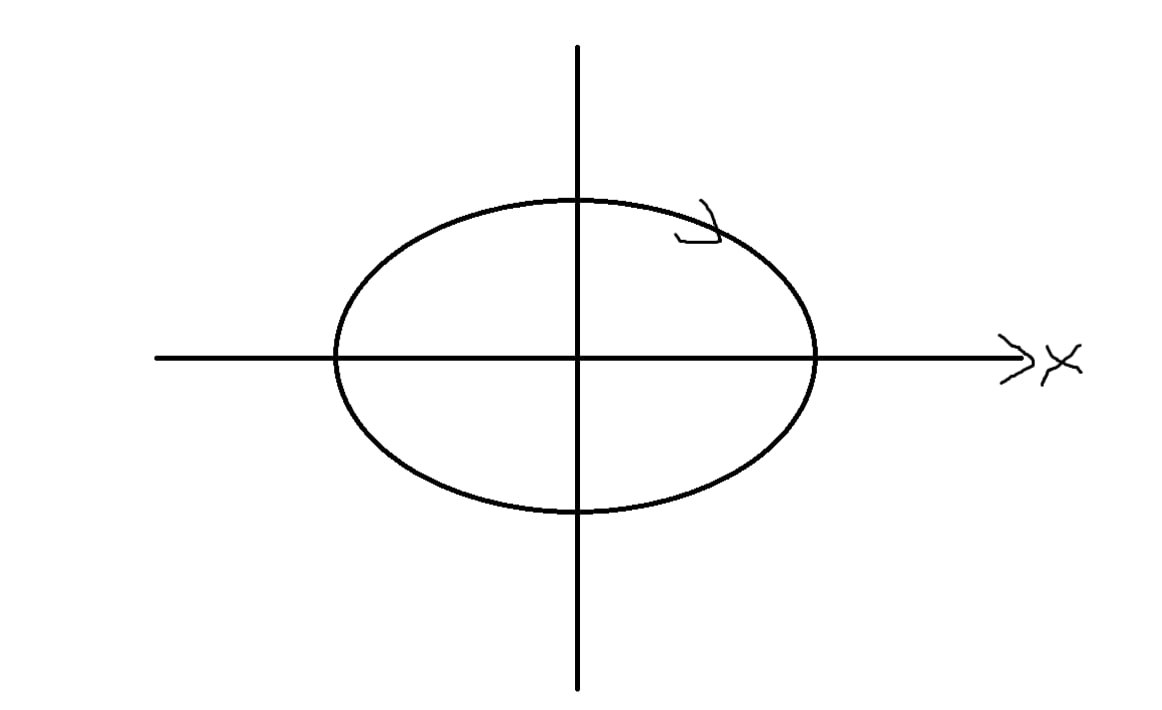
\includegraphics[width=15cm]{2.jpg}
	\caption{Эллипс поляризации для вектора $\bm{E}$, вышедшего из пластинки $\lambda/4$}
\end{figure}

\begin{figure}[H]
	\centering
	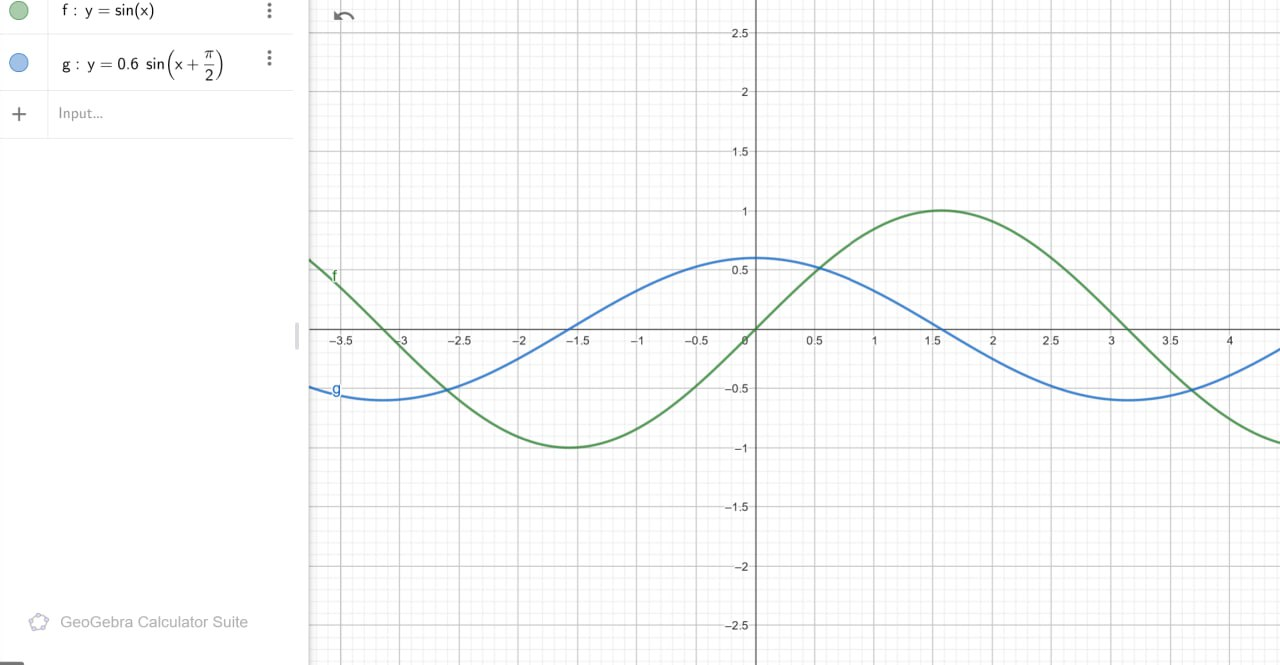
\includegraphics[width=15cm]{3.jpg}
	\caption{Картина колебаний полей со сдвигом фаз в $\pi/2$}
\end{figure}
\end{document}